\documentclass[aspectratio=169,xcolor=dvipsnames]{beamer}
\usetheme{Madrid}
\usecolortheme{seahorse}
\usepackage{amsmath,amssymb,booktabs,hyperref,listings,tikz}
\usetikzlibrary{arrows.meta,positioning,shapes}
\lstset{
  language=Python,
  basicstyle=\small\ttfamily,
  keywordstyle=\color{blue}\bfseries,
  commentstyle=\color{OliveGreen},
  stringstyle=\color{red},
  frame=single,
  breaklines=true
}

\title[Algorithms -- Week 3]{\textbf{Design and Analysis of Algorithms}\\
\large Week 3: Divide and Conquer Algorithms}
\subtitle{Paradigm Principles, Classical Sorting \& Recurrence Relations}
\author{Computer Science Curriculum Series}
\date{Lecture Slides}

\AtBeginSection[]{
  \begin{frame}<beamer>{Outline}
    \tableofcontents[currentsection]
  \end{frame}
}

\begin{document}

\begin{frame}
  \titlepage
\end{frame}

\begin{frame}{Outline}
  \tableofcontents
\end{frame}

% ==========================================
\section{The Divide and Conquer Paradigm}
% ==========================================

\begin{frame}{General Paradigm Design}
  **Divide and Conquer (D\&C)** is a fundamental algorithmic paradigm:
  \begin{description}
    \item[1. Divide:] Break the problem into a number of smaller subproblems that are **similar to the original** but smaller in size.
    \item[2. Conquer:] Solve the subproblems **recursively**. If the subproblem sizes are small enough (base case), solve them straightforwardly.
    \item[3. Combine:] **Merge** the solutions of the subproblems into the solution of the original problem.
  \end{description}
  \begin{block}{Recursive Complexity Form}
    Many D\&C algorithms partition a problem of size $n$ into $a$ subproblems, each of size $n/b$, with $\mathcal{O}(f(n))$ work to divide and combine:
    $$T(n) = a T(n/b) + f(n)$$
  \end{block}
\end{frame}

\begin{frame}{Why Divide and Conquer?}
  \begin{itemize}
    \item **Efficiency:** D\&C can reduce runtime bounds significantly (e.g., from $\mathcal{O}(n^2)$ sorting to $\mathcal{O}(n \log n)$).
    \item **Parallelizability:** Subproblems are often independent and can be solved concurrently.
    \item **Memory Friendliness:** Many D\&C algorithms exhibit high cache locality (locality of reference).
  \end{itemize}
  \begin{exampleblock}{Classical Success Stories}
    * **Merge Sort \& Quick Sort:** Optimal comparisons-based sorting ($\Theta(n \log n)$).
    * **Binary Search:** $\Theta(\log n)$ search on sorted arrays.
    * **Karatsuba Integer Multiplication:** $\Theta(n^{1.585})$ instead of $\Theta(n^2)$.
    * **Strassen's Matrix Multiplication:** $\Theta(n^{2.807})$ instead of $\Theta(n^3)$.
  \end{exampleblock}
\end{frame}

% ==========================================
\section{Merge Sort}
% ==========================================

\begin{frame}{Merge Sort: History \& Concept}
  \begin{itemize}
    \item Designed by **John von Neumann** in 1945.
    \item A perfect textbook implementation of Divide \& Conquer:
      \begin{description}
        \item[Divide:] Split the unsorted $n$-element array into two halves of size $n/2$.
        \item[Conquer:] Recursively sort both halves using Merge Sort.
        \item[Combine:] Linear-time **merge** operation to combine the two sorted halves into a single sorted array.
      \end{description}
  \end{itemize}
  \begin{block}{Recursive Halving}
    \begin{center}
    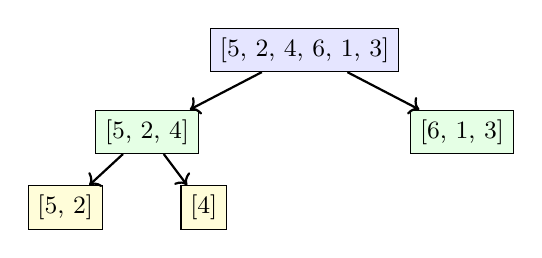
\begin{tikzpicture}[scale=0.8, font=\small]
      \node[draw, fill=blue!10] (root) at (4,2.5) {[5, 2, 4, 6, 1, 3]};
      \node[draw, fill=green!10] (L) at (1.5,1.2) {[5, 2, 4]};
      \node[draw, fill=green!10] (R) at (6.5,1.2) {[6, 1, 3]};
      \node[draw, fill=yellow!15] (LL) at (0.2,0) {[5, 2]};
      \node[draw, fill=yellow!15] (LR) at (2.4,0) {[4]};
      \draw[->, thick] (root) -- (L); \draw[->, thick] (root) -- (R);
      \draw[->, thick] (L) -- (LL); \draw[->, thick] (L) -- (LR);
    \end{tikzpicture}
    \end{center}
  \end{block}
\end{frame}

\begin{frame}[fragile]{Merge Sort: Algorithm Design}
  \begin{lstlisting}[language=Python]
def merge_sort(arr):
    if len(arr) <= 1:
        return arr                 # Base case
    mid = len(arr) // 2
    L = merge_sort(arr[:mid])      # Conquer left
    R = merge_sort(arr[mid:])      # Conquer right
    return merge(L, R)             # Combine

def merge(L, R):
    result = []
    i = j = 0
    while i < len(L) and j < len(R):
        if L[i] <= R[j]:           # <= preserves stability
            result.append(L[i]); i += 1
        else:
            result.append(R[j]); j += 1
    return result + L[i:] + R[j:]
  \end{lstlisting}
\end{frame}

\begin{frame}{Merge Sort: Complete Complexity Analysis}
  \begin{itemize}
    \item **Recurrence:** $T(n) = 2T(n/2) + \Theta(n)$
    \item **Time Complexity:** $\Theta(n \log n)$ in **all cases** (worst, average, best).
    \item **Space Complexity:** $\Theta(n)$ auxiliary space to perform the merges (not in-place).
    \item **Stability:** **Stable** (relative order of equal elements is preserved because of strict `L[i] <= R[j]` comparison).
  \end{itemize}
  \begin{block}{Merge Sort Recursion Tree}
    At level $k$, there are $2^k$ subproblems, each of size $n/2^k$.
    * Cost at each level $k$ is $2^k \times c(n/2^k) = cn$ work.
    * Height of the tree is $\log_2 n$.
    * Total cost: $\sum_{k=0}^{\log n} cn = cn \log_2 n = \Theta(n \log n)$.
  \end{block}
\end{frame}

% ==========================================
\section{Quick Sort}
% ==========================================

\begin{frame}{Quick Sort: Concept}
  * Designed by **Tony Hoare** in 1959.
  * A highly popular in-place sorting algorithm:
    \begin{description}
      \item[Divide:] Select a **pivot** element and **partition** the array such that:
        * All elements less than or equal to pivot are on the left.
        * All elements greater than pivot are on the right.
      \item[Conquer:] Recursively sort the left and right subproblems.
      \item[Combine:] Trivial! The array is sorted in-place during partitioning, so no combine step is needed.
    \end{description}
  \begin{block}{Key Difference from Merge Sort}
    * **Merge Sort:** Easy divide (split in half), hard combine (linear merge).
    * **Quick Sort:** Hard divide (in-place partition), easy combine (no-op).
  \end{block}
\end{frame}

\begin{frame}[fragile]{Quick Sort: Lomuto Partitioning}
  \begin{lstlisting}[language=Python]
def partition(arr, lo, hi):
    pivot = arr[hi]            # Pick last element as pivot
    i = lo - 1                 # Boundary index of smaller elements
    for j in range(lo, hi):
        if arr[j] <= pivot:
            i += 1
            arr[i], arr[j] = arr[j], arr[i]
    arr[i+1], arr[hi] = arr[hi], arr[i+1] # swap pivot into place
    return i + 1

def quicksort(arr, lo=0, hi=None):
    if hi is None: hi = len(arr) - 1
    if lo < hi:
        p = partition(arr, lo, hi)
        quicksort(arr, lo, p - 1)
        quicksort(arr, p + 1, hi)
  \end{lstlisting}
\end{frame}

\begin{frame}{Quick Sort Complexity: Worst vs Average}
  \begin{columns}
    \column{0.48\textwidth}
    \begin{alertblock}{Worst Case: $\Theta(n^2)$}
      Occurs when partition is extremely unbalanced ($0$ elements vs $n-1$ elements).
      * **Triggers:** Already sorted or reverse-sorted input with last/first element pivot.
      * **Recurrence:** $T(n) = T(n-1) + \Theta(n)$
    \end{alertblock}
    \column{0.48\textwidth}
    \begin{exampleblock}{Average Case: $\Theta(n \log n)$}
      Occurs when partition yields a reasonable split (even a $9$-to-$1$ split is asymptotically optimal!).
      * **Expected Comparisons:** $\approx 1.39 n \log_2 n$.
      * **Random Pivot:** Makes worst case practically impossible.
    \end{exampleblock}
  \end{columns}
  \vspace{0.5em}
  **Quick Sort Properties:**
  * **In-place:** Uses $\mathcal{O}(\log n)$ stack space (ignoring stack, $\mathcal{O}(1)$ auxiliary space).
  * **Unstable:** Swapping elements across the pivot boundary can break stability.
\end{frame}

% ==========================================
\section{Solving Recurrence Relations}
% ==========================================

\begin{frame}{Solving Recurrent Forms}
  To evaluate recursive time complexities, we use three primary mathematical toolsets:
  \begin{description}
    \item[1. Substitution Method:] Guess the form of the solution, then use mathematical induction to prove it correct.
    \item[2. Recursion Tree Method:] Draw a tree of execution levels, sum the costs at each level, and sum all levels. Highly visual and intuitive.
    \item[3. Master Theorem:] A cookbook recipe providing immediate asymptotic bounds for standard recurrence forms.
  \end{description}
\end{frame}

\begin{frame}{The Master Theorem}
  For recurrences of the form $T(n) = aT(n/b) + f(n)$ where $a \ge 1$ and $b > 1$:
  \begin{block}{Case 1: $f(n) = \mathcal{O}(n^{\log_b a - \epsilon})$ for some $\epsilon > 0$}
    **Subproblem cost dominates:** $T(n) = \Theta(n^{\log_b a})$.
  \end{block}
  \begin{block}{Case 2: $f(n) = \Theta(n^{\log_b a})$}
    **Equal level cost distribution:** $T(n) = \Theta(n^{\log_b a} \log n)$.
  \end{block}
  \begin{block}{Case 3: $f(n) = \Omega(n^{\log_b a + \epsilon})$ for some $\epsilon > 0$, and regularity holds}
    **Combine/Divide cost dominates:** $T(n) = \Theta(f(n))$.
  \end{block}
\end{frame}

\begin{frame}{Master Theorem: Canonical Examples}
  * **Merge Sort:** $T(n) = 2T(n/2) + \Theta(n)$
    * $a = 2, b = 2 \Rightarrow n^{\log_b a} = n^1 = n$.
    * Since $f(n) = \Theta(n)$, this falls under **Case 2**.
    * **Result:** $T(n) = \Theta(n \log n)$.
  * **Binary Search:** $T(n) = T(n/2) + \Theta(1)$
    * $a = 1, b = 2 \Rightarrow n^{\log_b a} = n^0 = 1$.
    * Since $f(n) = \Theta(1)$, this falls under **Case 2**.
    * **Result:** $T(n) = \Theta(\log n)$.
  * **Strassen's Matrix Multiplication:** $T(n) = 7T(n/2) + \Theta(n^2)$
    * $a = 7, b = 2 \Rightarrow n^{\log_2 7} \approx n^{2.81}$.
    * Since $f(n) = n^2 = \mathcal{O}(n^{2.81 - \epsilon})$, this falls under **Case 1**.
    * **Result:** $T(n) = \Theta(n^{\log_2 7}) \approx \Theta(n^{2.81})$.
\end{frame}

% ==========================================
\section{Advanced D\&C Applications}
% ==========================================

\begin{frame}{Inversion Counting}
  \begin{block}{Problem Statement}
    An **inversion** in an array $A$ is a pair of indices $(i, j)$ such that $i < j$ but $A[i] > A[j]$.
    Count the total number of inversions in an unsorted array of size $n$.
  \end{block}
  \begin{itemize}
    \item **Brute Force:** Compare all pairs in $\mathcal{O}(n^2)$ time.
    \item **D\&C Strategy (Modified Merge Sort):**
      * Split array into left and right halves.
      * Count inversions inside left half recursively, and sort it.
      * Count inversions inside right half recursively, and sort it.
      * Count crossing inversions: when merging $L$ and $R$, if $L[i] > R[j]$, then all remaining elements in sorted $L$ are also larger than $R[j]$ (adds $len(L) - i$ to inversion count).
      * **Complexity:** $\mathcal{O}(n \log n)$ time, $\mathcal{O}(n)$ space.
  \end{itemize}
\end{frame}

\begin{frame}{Maximum Subarray Sum}
  \begin{block}{Problem Statement}
    Find the contiguous subarray within a one-dimensional array of numbers $A[0 \ldots n-1]$ which has the largest sum.
  \end{block}
  \begin{description}
    \item[Divide:] Split the array into two equal halves.
    \item[Conquer:] Find maximum subarray sum entirely in the left half, and entirely in the right half recursively.
    \item[Combine:] Find the maximum subarray that **crosses** the middle point. This can be done in linear $\mathcal{O}(n)$ time by scanning outward from the center.
  \end{description}
  * **Recurrence:** $T(n) = 2T(n/2) + \Theta(n)$
  * **Time Complexity:** $\Theta(n \log n)$ via Case 2 of Master Theorem.
\end{frame}

\begin{frame}{Summary \& Practical Sorting}
  \begin{itemize}
    \item D\&C algorithms successfully partition hard tasks into independent subproblems.
    \item **Merge Sort** provides guaranteed $\Theta(n \log n)$ time and stable sorting, at the cost of linear extra memory.
    \item **Quick Sort** sorts in-place but requires careful pivot selection to guarantee expected $\Theta(n \log n)$ time.
    \item **Practical Hybrid Sorts:**
      * **Timsort:** Combines Merge Sort and Insertion Sort. Used in Python and Java.
      * **Introsort:** Starts with Quicksort, switches to Heapsort if recursion depth exceeds a threshold, and uses Insertion Sort for small partitions. Used in C++ STL.
  \end{itemize}
\end{frame}

\end{document}
